%-------------------------------------------------------------------------------
% pattern_editor
%-------------------------------------------------------------------------------
%
% \file        pattern_editor.tex
% \library     Documents
% \author      Chris Ahlstrom
% \date        2015-08-31
% \update      2021-10-16
% \version     $Revision$
% \license     $XPC_GPL_LICENSE$
%
%-------------------------------------------------------------------------------

\section{Pattern Editor}
\label{sec:pattern_editor}

   The \textsl{Seq66} \textbf{Pattern Editor} can edit and preview a
   pattern, configure its buss, channel, transpose, musical
   scale, and many other settings.
   A slightly modified  version of the \textbf{Pattern Editor} appears in the
   \textbf{Edit} tab in the main window; the main window has to be expanded
   vertically to see all of the controls.
   The complete version can be brought up in an external window.

\begin{figure}[H]
   \centering 
   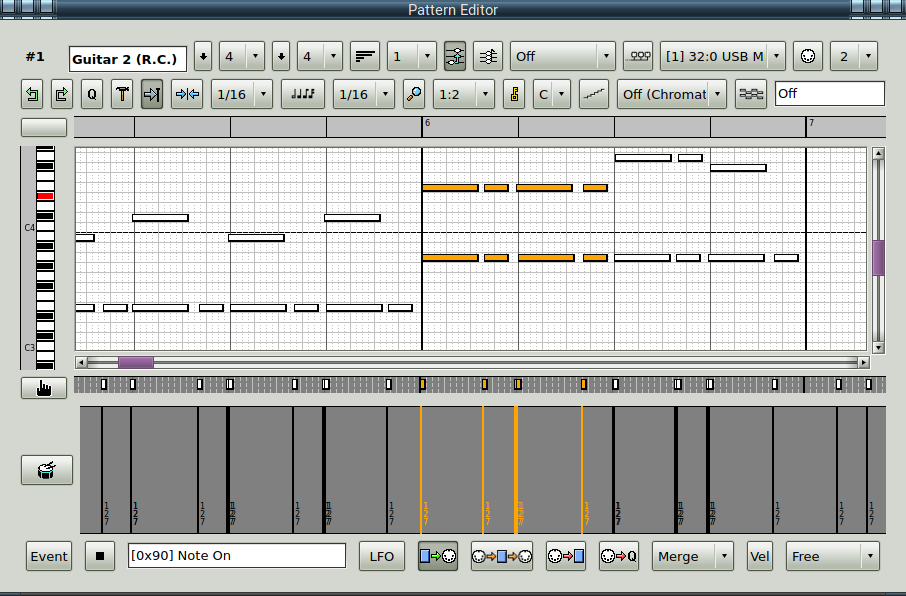
\includegraphics[scale=1.00]{pattern-editor/pattern-edit-window.png}
   \caption{External Pattern Editor Window}
   \label{fig:pattern_editor_window}
\end{figure}
  
   The \textbf{Pattern Editor} is complex, and we will discuss the external
   window only since its features are a superset of the \textbf{Edit} tab.
   For exposition, we break the window into the following sections:

   \begin{enumber}
      \item \textbf{First Row}
      \item \textbf{Second Row}
      \item \textbf{Time}
      \item \textbf{Piano Roll}
      \item \textbf{Events}
      \item \textbf{Data Panel}
      \item \textbf{Bottom Row}
      \item \textbf{Common Actions}
   \end{enumber}

   Before we describe this window, there are some things to recognize.
   First, if the pattern is empty when play is started, the progress bar will
   still move, so that the user can play a MIDI instrument and record new notes.
   Second, to add a note with the mouse, one must press the \textsl{right}
   mouse button (the pointer changes to a pencil) and,
   \textsl{while holding it}, press the left mouse button.
   Or click in the pattern editor, press the
   \index{keys!p}
   \texttt{p} key to select the "pencil" or "paint" mode, then
   \index{mouse!left-click}
   left-click to add a note or
   \index{mouse!left-click-drag}
   left-click-drag to add multiple notes as the mouse moves.
   \index{keys!x}
   Press or release the right mouse button, or press
   \texttt{x} to "eXit" or "eXscape" from paint mode.
   Another option is to press the "finger" button to toggle between note-entry
   and note-selection.
   Third, notes are drawn only with the length selected by the "notes" button
   near the top of the pattern window.  There are tricks to
   modifying the new notes that are described later.

   \textsl{Seq66} automatically scrolls
   horizontally through the sequence/pattern editor window when
   playback moves the progress bar outside of the current frame of data.  This
   feature makes it easier to follow patterns that are longer than a measure or
   two.

   One might want to print out the following figure to follow along.  There is
   a lot of functionality in this window.

\begin{figure}[H]
   \centering 
   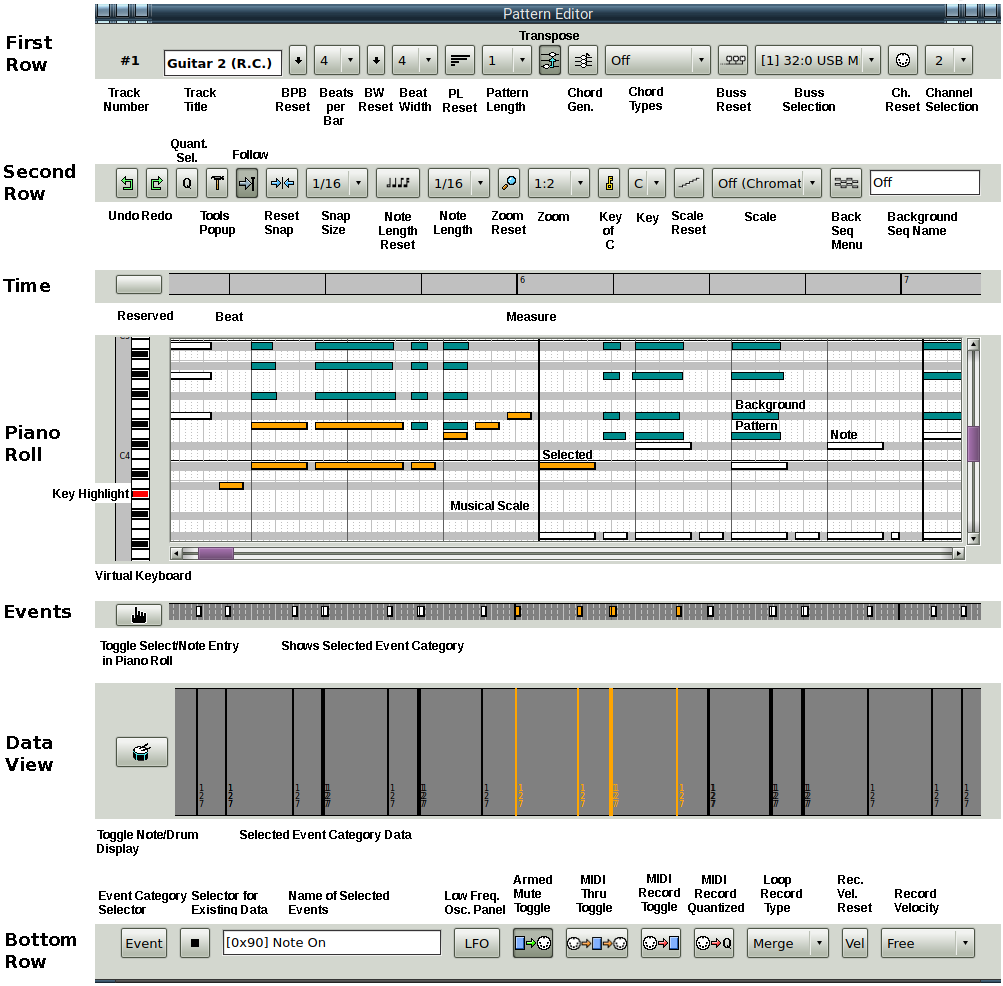
\includegraphics[scale=0.90]{pattern-editor/pattern-edit-window-annotated.png}
   \caption{Pattern Editor Window, Annotated}
   \label{fig:pattern_editor_window_annotated}
\end{figure}

\subsection{Pattern Editor / First Row}
\label{subsec:pattern_editor_first_row}

   The top bar (horizontal panel) of the Pattern (sequence) Editor
   lets one change the name of
   the pattern/loop/sequence/track, the time signature of the piece, how long
   the track is, and some other configuration items.

   \begin{enumber}
      \item \textbf{Track Number}
      \item \textbf{Track Title}
      \item \textbf{Beats Per Bar Reset} and \textbf{Beats Per Bar}
      \item \textbf{Beat Width Reset} and \textbf{Beat Width}
      \item \textbf{Pattern Length Reset} and \textbf{Pattern Length}
      \item \textbf{Chord Types}
      \item \textbf{Buss Reset} and \textbf{Buss Selection}
      \item \textbf{Channel Reset} and \textbf{Channel Selection}
   \end{enumber}

   \setcounter{ItemCounter}{0}      % Reset the ItemCounter for this list.

   \itempar{Track Number}{pattern editor!number}
   This item shows the sequence/track/pattern/loop
   number, to make it easier to pick it out when a lot of patterns are being
   edited at once.

   \itempar{Track Name}{pattern editor!name}
   Provides the name of the pattern.
   This name should be short and memorable.
   It is displayed in the \textbf{Live Grid} (the \textbf{Patterns Panel}),
   on the top line of its pattern slot.

   \itempar{Beats Per Bar}{pattern editor!beats/bar}
   \index{beats per bar}
   Specifies the number of beat units per bar in the time signature.
   The possible values range from 1 to 16, if the drop-down menu is used.
   Arbitrary values up to 32 can be entered by typing the number.
   The "Reset" button resets the value to 4.

   \itempar{Beat Width}{pattern editor!beat width}
   \index{beat width}
   Specifies the size of the bottom beat unit of the time signature:
   1 for whole notes; 2 for half notes; 4 for quarter notes; 8 for eight notes;
   16 for sixteenth notes; and 32 for thirty-second notes.
   The whole time signature is display at the bottom center of the
   corresponding pattern slot in the \textbf{Live Grid}.
   Arbitrary values up to 32 can be entered by typing the number.
   The "Reset" button resets the value to 4.

   \itempar{Pattern Length}{pattern editor!length}
   Sets the length of the current pattern, in measures.
   The possible values range from 1 to 64.
   Arbitrary values up to 1024 can be entered by typing the number.
   \textsl{However}, when opening or importing a non-\textsl{Seq66}
   MIDI tune, the length of each track will be used, and so other values
   are possible.

   Bringing up a pattern less than one measure or bar in
   length in the pattern editor will adjust the pattern to pad it to the
   length of one measure.
   \index{pattern editor!progress bar}
   \textsl{Seq66} will, when it reads such a short pattern
   from a MIDI file,

   A feature from user \textsl{stazed} allows the pattern to expand
   indefinitely while the user inputs MIDI from a controller, via the
   \textbf{Expand} option of the \textbf{Loop Record Type}.

%  See \sectionref{subsec:pattern_editor_bottom} below.

%  WHAT IS THIS? A feature where a short loop plays only once.
%
%  (Also nice would be a "one-shot"
%  pattern, useful for live intro patterns, for example.)

   \itempar{Chord Types}{pattern editor!chord types}
   \index{chord generation}
   This setting allows one to select a chord type (e.g. "major" or "minor").
   When active, a note is treated like the base note of the selected chord
   type, and extra notes are generated to create that chord.
   The \textbf{Chord Generation Reset} button is at the left of the
   \textbf{Data Panel}.

   \itempar{Chord Generation}{pattern editor!chord generation}
   \index{chord generation}

   \itempar{MIDI Out Device (Buss)}{pattern editor!midi out device}
   This setting specifies a virtual MIDI output buss or a
   MIDI output device set up by the computer and
   attached MIDI equipment.
   The button resets it to buss 0.
   Note that, if the pattern's selected buss is not found, this entry will be
   blank.  The user must select a valid buss from this dropdown.

   \itempar{MIDI Out Channel}{pattern editor!midi out channel}
   The \textbf{Channel Selection} setting selects the MIDI output channel.
   The possible values range from 1 to 16, plus \textsl{Free}, which means
   that the channels of the events are preserved, and are used as the output
   channel, a bit like an SMF 0 track.
   The editing channel is always channel 1.
   If instruments are assigned in the 'usr' configuration file
   to that device and channel, their names will be shown in the dropdown.

   In addition, this setting determines the channel applied when painting notes
   in the piano roll.  If set to "1" or "Free" (no channel), then channel 1 is
   applied.  Otherwise, if set to "2" through "16", that channel is applied.

\subsection{Pattern Editor / Second Row}
\label{subsec:pattern_editor_second_row}

   The second horizontal panel of the Pattern Editor provides a number
   of additional settings and functions:

   \begin{enumber}
      \item \textbf{Undo}
      \item \textbf{Redo}
      \item \textbf{Quantize Selection}
      \item \textbf{Tools Popup}
      \item \textbf{Follow Progress}
      \item \textbf{Reset Snap} and \textbf{Grid Snap}
      \item \textbf{Note Length Reset} and \textbf{Note Length}
      \item \textbf{Zoom Reset} and \textbf{Zoom}
      \item \textbf{Key Reset} and \textbf{Key of Sequence}
      \item \textbf{Scale Reset} and \textbf{Musical Scale}
      \item \textbf{Background Sequence}
   \end{enumber}

   \setcounter{ItemCounter}{0}      % Reset the ItemCounter for this list.

   \itempar{Undo}{pattern editor!undo}
   The \textbf{Undo} button rolls back any changes to the pattern from this
   session.  It will roll back one change each time pressed.
   \index{keys!ctrl-z}
   Pressing \texttt{Ctrl-Z} is the same as using the \textbf{Undo} button.

   \itempar{Redo}{pattern editor!redo}
   The \textbf{Redo} button will restore any undone changes to the pattern from
   this session.
   It will restore one change each time it is pressed.
   There is currently no redo key.

   \itempar{Quantize Selection}{pattern editor!quantize}
   This button quantizes the selected events as per
   the \textbf{Grid Snap} setting.

   \itempar{Tools}{pattern editor!tools}
   This button brings up a nested menu of tools for modifying selected
   events and notes:

   \begin{enumber}
      \item \textbf{Select}.  This menu provides two note-selection options:
         \begin{itemize}
            \item \textbf{Select all}, selects all notes in the pattern;
               The \index{keys!ctrl-a} \texttt{Ctrl-A} will also select
               all of the events in the pattern editor.
            \item \textbf{Inverse selection}, which inverts the selection of
               notes.
         \end{itemize}
      \item \textbf{Timing}. This menu
            offers two ways to tweak the timing of the selected note:
         \begin{itemize}
            \item \textbf{Quantize}
               \index{quantize}
               quantizes the selected notes, the same way as the
               \textbf{Quantize} ("\textbf{Q}") button.
            \item \textbf{Tighten},
               \index{tighten}
               which is merely a less strict form of quantization.
         \end{itemize}
      \item \textbf{Pitch transpose} allows uniform transpostion
         regardless of the key and scale in force for the pattern.
         \index{modify pitch}
         Selecting this item entry brings up a sub-menu.
      \item \textbf{Harmonic Transpose Selected}, which makes sure
         that all transpositions stay on the selected scale.
         If the scale selection is off, this is the same as plain pitch
         transpose.
   \end{enumber}

   \itempar{Follow Progress}{pattern editor!tools}
   This button toggles whether or not the progress bar follows
   progress in long patterns.  Turning off this feature is useful when
   one wants to concentrate on the current measure without the paging to
   subsequent measures that occurs with the "follow progess" feature.

   \itempar{Grid Snap}{pattern editor!grid snap}
   Grid snap selects where the notes will snap when
   \textsl{drawn} and when \textsl{moved} (but not when lengthened/shortenend).
   That is, it selects the snap-spacing for the notes
   The following values are supported:
   \textbf{1}, \textbf{1/2}, \textbf{1/4}, \textbf{1/8},
   \textbf{1/16} (\textsl{the default value}),
   \textbf{1/32}, \textbf{1/64}, and \textbf{1/128}.
   Additional values are also supported:
   \textbf{1/3}, \textbf{1/6}, \textbf{1/12}, \textbf{1/24},
   \textbf{1/48}, \textbf{1/96}, and \textbf{1/192}.
   The button to the left of this control resets it to the default value.

   \itempar{Note Length}{pattern editor!note length}
   Note length determines the duration of inserted notes.
   Like the \textbf{Grid Snap} values,
   the following values are supported:
   \textbf{1}, \textbf{1/2}, \textbf{1/4}, \textbf{1/8},
   \textbf{1/16} (\textsl{the default value}),
   \textbf{1/32}, \textbf{1/64}, and \textbf{1/128}.
   Additional values are also supported:
   \textbf{1/3}, \textbf{1/6}, \textbf{1/12}, \textbf{1/24},
   \textbf{1/48}, \textbf{1/96}, and \textbf{1/192}.
   The button to the left of this control resets it to the default value.

   \itempar{Zoom}{pattern editor!zoom}
   Horizontal zoom is the ratio between MIDI pixels and ticks, written as
   "pixels:ticks", where "ticks" is the "pulses" in "PPQN".
   For example, 1:4 = 4 ticks per pixel.
   Supported values are
   \textbf{1:1}, \textbf{1:2} (\textsl{the default value}),
   \textbf{1:4}, \textbf{1:8}, \textbf{1:16},
   and \textbf{1:32}, along with
   more values to support higher PPQN tunes:
   \textbf{1:64}, \textbf{1:128}, \textbf{1:256}, and \textbf{1:512}.
   The default zoom is 2 for the standard PPQN value, 192, but it
   increases for higher PPQN values, so that the default zoom looks sensible.
   As the right number (ticks) goes higher,
   the effect is to zoom out, and show more of the pattern.
%  Also see \sectionref{subsubsec:pattern_editor_zoom_keys}.

   \itempar{Key of Sequence}{pattern editor!key}
   Selects the desired musical key for the pattern.  The following keys are
   supported:
   \textbf{C}, \textbf{C\#},
   \textbf{D}, \textbf{D\#},
   \textbf{E}, \textbf{F}, \textbf{F\#},
   \textbf{G}, \textbf{G\#},
   \textbf{A}, \textbf{A\#},
   and \textbf{B}.
   Changing the key shifts the marked note-rows
   for the \textbf{Musical Scale} setting and indicates the base notes
   of the key in a \textbf{bold} font.
   The small key button resets the key to \textbf{C}.

   \index{save musical key}
   The musical key that a sequence/pattern is set to is
   saved in the MIDI file along with the rest of the data for the sequence.
   \textbf{However},
   a change made to the key, scale, or background sequence in
   the pattern editor can be saved in the whole song,
   so that opening another sequence
   will apply the same settings to that sequence.  This is an optional feature,
   supported as noted below.

   Also see \textbf{Musical Scale} below for the scale-identification feature.

   \index{global-sequence}
   If the global-sequence feature is enabled, and the user selects
   a different key, scale, or background sequence in the pattern editor, 
   then \textsl{all} patterns share the selected key, scale, or background
   sequence.  Furthermore, these settings are saved in the "proprietary"
   section of the MIDI file, where they are available for all patterns.

   If the global-sequence feature is \textsl{not} enabled, and the user selects
   a different key, scale, or background sequence in the pattern editor, 
   then only that pattern will use the selected key, scale, or background.
   The key, scale, or background sequence change will be saved in the MIDI file
   only for that pattern, as a SeqSpec meta event.
   The global-sequence feature setting can be made in the 'usr' configuration
   file.

   \itempar{Musical Scale}{pattern editor!scale}
   Selects the desired background scale for the pattern; it provides a way for
   someone to key in notes that are only in that scale.
   When a scale is selected, the following features are supported:

   \begin{itemize}
      \item The notes that are \textsl{not}
         in the scale are shown as grey in the piano roll.
      \item For harmonic transposition, the notes are shifted
         so that they remain in the selected scale.
      \item The exact notes that are considered "in-scale" shift according
         to the value of the selected \textbf{Key of Sequence}.
   \end{itemize}

   \index{musical scales}
   The following musical scales are supported so far:

   \begin{itemize}
      \item \textbf{Off (Chromatic)}
      \item \textbf{Major (Ionian)}
      \item \textbf{Minor (Aeolian)}
      \item \textbf{Harmonic Minor}
      \item \textbf{Melodic Minor}
      \item \textbf{Whole Tone}
      \item \textbf{Blues}
      \item \textbf{Major Pentatonic}
      \item \textbf{Minor Pentatonic}
      \item \textbf{Phrygian}
      \item \textbf{Enigmatic}
   \end{itemize}

   Please let us know of any mistakes in these scales.
   Note that the \textbf{Melodic Minor} scale is supposed to
   descend in the same way as the natural \textbf{Minor} scale, but
   there is no way to support that trick in \textsl{Seq66}.

   One can select which \textbf{Musical Scale} and
   \textbf{Key} the piece is in nominally,
   and \textsl{Seq66} will grey those keys on the piano-roll that
   are \textsl{not} in the selected scale for the selected key.
   This is purely visual; a user can still add off-key notes.
   This feature makes it easier to stay in key while playing and recording.
   The scale will shift when a different \textbf{Key} is selected.

   \index{save musical scale}
   The scale that a pattern is set to is
   saved in the MIDI file along with the rest of the data for the pattern.
   A change made to the key, scale, or background pattern in
   the pattern editor can be saved globally, so that opening another pattern
   apply the same settings to that pattern.  This is a configurable feature in
   the 'usr' file; see "global\_seq\_feature".
   This option allows applying the key/scale/background-sequence
   either globally (all patterns) or locally (per-pattern), with each pattern
   holding its key, scale, and background-sequence settings in
   SeqSpec meta events.

   \index{scale identifier}
   \index{keys!ctrl-k}
   The pattern editor's piano roll has a little secret:
   the \textbf{Scale Identifier}.
   When the piano roll has focus and \texttt{Ctrl-K} is pressed,
   all of the notes in the pattern are analyzed to try to determine
   the both the key and the scale of the existing notes.
   The method is not sophisticated... the notes are counted and are matched
   against all of the keys (C to B) and scales supported by \textsl{Seq66}.
   The combinations with the highest number of notes are then shown in a
   message box.
   This simple analysis depends on having at least 8 notes in the pattern, and
   it is possible to get weird results if
   there are only a few \textsl{different}
   notes, as in a simple bass line.
   Don't expect miracles from this feature.
   A more sophisticated analysis, the
   \textsl{Krumhansl-Schmuckler} key-finding
   algorithm, could be used, but it is a bit too complex
   for our needs, which are basic.

   \itempar{Background Sequence}{pattern editor!background sequence}
   One can select another pattern to draw on the background to help with
   writing corresponding parts.
   The button brings up a small menu with values of \textbf{Off} and
   \textbf{Set 0} (at a minimum).
   The 0 is a set number; sets are numbered from 0 to 31.
   Additional set numbers appear in the menu for each set that has data in it.
   Under the \textbf{Set 0} entry, a menu appears.
   Once the desired pattern is selected from that list, it appears as dark cyan
   note bars, along with the normal notes that are part of the pattern.

   \index{save background sequence}
   The background sequence that shows is saved in the MIDI file
   along with the rest of the data for the sequence/pattern.
   A change made to the key, scale, or background sequence in
   the pattern editor is saved in the editor, so that opening another sequence
   will apply the same settings to that sequence.
   This is an optional feature, as noted earlier.

   \itempar{Chord Generation}{pattern editor!chord generation}
   One can insert chords with one click.
   (This feature comes from user "stazed"
   and his \textsl{Seq32} project \cite{seq32}.)
   Select the desired chord type first.
   Once a value other than \textbf{Off} is selected,
   drawing mode will add multiple notes representing the chord
   created, with the clicked note value as the base of the chord.

\subsection{Pattern Editor / Time}
\label{subsec:pattern_editor_time}

   The following are the elements of the \textbf{Time} line:

   \begin{itemize}
      \item \textbf{Vertical Zoom Buttons}.
         These buttons allow the user to compress, reset, or expand the
         piano roll vertically to a certain degree.  A more permanent change
         can be made by setting the \textbf{Editor Key Height} value in
         the \textbf{Edit / Preferences / Display} tab, or in the 'usr' file.
      \item \textbf{Time Line}.
         The \textbf{Time} (or \textbf{Measures}) bar provides an explicit
         count of beats and bars.
         It follows the horizontal zoom of the piano roll.
         It also has a couple tricks:
         \begin{itemize}
            \item \textbf{In the upper half} of the time-line,
               the mouse pointer changes to a vertical pointer.
               Clicking there then shows a vertical bar and a dot; these mark
               the starting position of playback.
               This is useful for reviewing some notes.
            \item \textbf{In the lower half} of the time-line,
               the mouse pointer changes to a "finger" icon.
               Left-clicking there then moves the "L" marker to that point.
               Right-clicking there moves the "R" marker to that point.
               ("R" will never precede "L", though).
               If the \textbf{Loop} button in the main window is active, then
               playback will loop between the "L" and "R" buttons.
               This looping now works with both Live and Song modes.
         \end{itemize}
   \end{itemize}

\subsection{Pattern Editor / Piano Roll}
\label{subsec:pattern_editor_piano_roll}

   The piano roll is the center of the pattern/loop/track/sequence editor.
   It is accompanied by a thin "event bar" ("event area", "event strip")
   just below it,
   and a taller "data bar" or "data area" just below that.
   While the pattern
   editor is very similar to note editors in other sequencers, it is a bit
   different in feel.  A good mouse with at least 3 buttons is very helpful
   for editing.  Buttons and keystrokes enhance the ease of editing.

   The piano roll can show notes, a background pattern, and a scale.
%  and tempo events.
   Notes are shown as narrow rectanges; the pattern and scale are
   shown as bars running the whole length of the piano roll.
%  Tempo events are shown as small circles accompanied by a number.
%  (We're still considering whether showing tempos in the piano roll is a good
%  thing).

   When the piano roll has keyboard focus, the \texttt{Space} key
   starts and stops playback, rewinding to the beginning when stopped.
   The \texttt{.} (period) key starts and pauses playback, without
   rewinding.
   The \texttt{Esc} key stops playback.
   This functionality is similar to that of the main window, but
   these keys are not reconfigurable in the piano roll.

   One can page vertically in the piano roll using the
   \index{keys!page-up} \texttt{Page Up} and 
   \index{keys!page-down} \texttt{Page Down} keys.
%  One can go to the top using the 
%  \index{keys!home} Home key, and
%  to the bottom using the
%  \index{keys!end} End key.
   One can go to the leftmost position using the 
   \index{keys!ctrl-home} \texttt{Ctrl-Home} key,
   and to the rightmost position using the
   \index{keys!ctrl-end} \texttt{Ctrl-End} key,

   \index{keys!arrows}
   If no notes are selected, the arrow keys will move the piano row up, down,
   left, and right.
   \index{keys!hjkl}
   In addition, the "vi" keys \texttt{h}, \texttt{j}, \texttt{k}, and
   \texttt{l} will act like the arrow keys. This can be convenient, especially
   if the arrow-keys are unwieldly.  For example, the
   \textsl{Microsoft Arc} keyboard puts all four arrows on one button!

   \index{step}
   \index{note step}
   With the note-step feature, if one paints notes with the mouse,
   the note position advances with each click.
   If one paints notes via an external MIDI keyboard, the notes are painted and
   advanced.
   To preview notes entered via a MIDI device, click the
   \textbf{MIDI Thru} button to activate so that they will be
   passed to the sound generator or software synthesizer.

\subsubsection{Pattern Editor / Piano Roll Items}
\label{subsubsec:pattern_editor_piano_roll_items}

   The center of the pattern editor consists of a time panel at the top,
   a virtual keyboard at the left, a note grid, a vertical scrollbar, an event
   panel, and a data panel at the bottom.

   \begin{enumber}
      \item \textbf{Beat}
      \item \textbf{Measure}
      \item \textbf{Virtual Piano Keyboard}
      \item \textbf{Notes}
   \end{enumber}

   \setcounter{ItemCounter}{0}      % Reset the ItemCounter for this list.

   \itempar{Beat}{piano roll!beat}
   The light vertical lines represent the beats defined by the configuration
   for the pattern.  The even lighter dotted lines between the beats are useful
   for snapping notes.

   \itempar{Measure}{piano roll!measure}
   The heavy vertical lines represent the measures (bars) defined by the
   configuration for the pattern.
   \index{pattern!end marker}
   Also note that the end of the pattern
   occurs at the end of a measure, and is marked by a blocky \textbf{END}
   marker.

   \itempar{Virtual Piano Keyboard}{piano roll!virtual piano keyboard}
   The virtual keyboard is a fairly powerful interface.  It shows,
   by shadowing, which note on the keyboard will be drawn. It can be
   played with a mouse, using left-clicks, to preview a short motif.
%  It can show marks to indicate off-scale notes, to make them easy to
%  avoid.
   Every octave, a note letter and octave number are shown, as in
   "C4".  If there is a difference scale in force, then the letter changes to
   match, as in "F\#5".

   \index{virtual keyboard!right-click}
   A right-click in the virtual keyboard area toggles the display
   between octave-note letters, MIDI note-numbers, and other views.
   The following figure shows all views, superimposed for comparison.

\begin{figure}[H]
   \centering 
   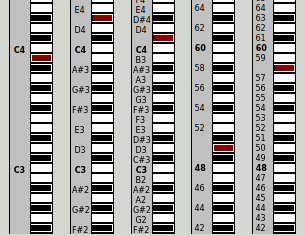
\includegraphics[scale=1.00]{pattern-editor/pattern-edit-window-key-numbers.png}
   \caption{Virtual Keyboard Number and Note Views}
   \label{fig:pattern_editor_key_numbers}
\end{figure}

   \itempar{Notes}{piano roll!notes}
   Musical notes are indicated in the piano roll
   by thick horizontal bars with white
   centers.  Each bar provides
   a visual representation of the pitch of a note and the length of a note.
   The current scale and background pattern can also be shown in the piano
   roll.

   \itempar{Time Scroll}{pattern editor!time scroll}
   Allows one to pan through the whole pattern, if it is too long to fit in
   the window horizontally.

\subsubsection{Pattern Editor / Note Painting}
\label{subsubsec:pattern_editor_note_painting}

   When we say "editing" in the context of the piano roll, in part we mean that
   we will "draw"
   \index{draw mode}
   \index{mode!draw}
   \index{paint mode}
   \index{mode!paint}
   or "paint" notes.
   Drawing, modifying, copying, and deleting notes is fairly easy in
   \textsl{Seq66}, though a little different from other MIDI sequencers.

   The \textsl{Seq24} note-editing style is as expected for basic
   actions such as selecting and moving notes using the left mouse button.
   Drawing a note or event is a bit different, in that one must first
   enter the drawing mode ("paint mode").
   One way is to \textsl{click and hold} the right mouse button, and then
   \textsl{click and drag} the mouse to insert notes.
   Note that some \textsl{Seq66} windows
   can use the \textsl{Ctrl-left-click} as a middle click. 
   \index{keys!p}
   Another way is to use the \texttt{p} key to enter the "paint" mode.
   To get out of the "paint" mode, press the
   \index{keys!x}
   \texttt{x} key while in the sequence editor.
   Also available is a "finger" button
   (\textbf{Note Select/Note Entry})
   to click to toggle the mode.

   \index{notes!inserting}
   Notes are inserted to be at the current length and grid-snap values for
   the sequence editor for as long as the buttons are pressed while the mouse
   is dragged.
   The length of the note will
   be that specified in the note-length setting (e.g. "1/16").
   \index{auto-note}
   This is the "auto-note" feature.
   The auto-note feature also works with chord-generation.
   Notes are inserted only up to the specified sequence length.
   Once notes are inserted, moving the mouse with the left button still
   held down moves the notes to the new note value of the mouse.
   If one releases the left button, then presses and holds it again,
   more notes will be added in the same way.
   This is a good way to layer notes in a short sequence.
   The draw mode has the following features:

   \begin{itemize}
      \item Notes are continually added as the mouse is dragged ("auto-notes").
      \item Notes cannot be added past the "END" marker of the pattern, which
         marks the \textbf{Sequence Length in bars} setting.
      \item As the mouse is dragged while the left button is held in draw mode,
         notes are either added, or, if already present at that note-on time,
         are moved up and down.
      \item If the draw mode is exited, and entered again, then the original
         notes will not be altered.  Instead, new ones will be added.
      \item Notes can be added while the pattern is playing, and will be heard
         the next time the progress bar passes over them.
   \end{itemize}

   Drawing/painting can also be done while the sequence is playing,
   and notes will be added to be played the next time the progress bar crosses
   them.

\subsubsection{Pattern Editor / Note Editing}
\label{subsubsec:pattern_editor_note_editing}

   Once notes are in place, whether by recording or using "paint" mode,
   the piano roll provides a sophisticated set of note-editing
   actions.

   \setcounter{ItemCounter}{0}      % Reset the ItemCounter for this list.

   \itempar{Event Selection}{event!select}
   There are various ways to select events and copy, delete, or modify them
   using the mouse or the keyboard in the piano roll:

   \begin{itemize}
      \item
         \index{keys!ctrl-a}
         \index{selection!all}
         \textbf{\texttt{Ctrl-A}}.
         Pressing the \texttt{Ctrl-A} key will select all of the events in the
         pattern editor.
      \item
         \index{keys!ctrl-e}
         \index{selection!events by channel}
         \textbf{\texttt{Ctrl-E}}.
         Pressing the \texttt{Ctrl-E} key will select all of the events in the
         pattern editor that have the channel that is selected in the
         channel dropdown.
         This selection is useful if one wants to move events from one channel
         into another pattern.
      \item
         \index{keys!ctrl-n}
         \index{selection!notes by channel}
         \textbf{\texttt{Ctrl-N}}.
         Pressing the \texttt{Ctrl-N} key will select all of the notes
         in the pattern editor that have the channel that is selected in the
         channel dropdown.
         This selection is useful if one wants to move notes from one channel
         into another pattern.
      \item
         \index{mouse!left-click}
         \index{pattern editor!left click}
         \index{pattern editor!select note}
         \textbf{Left Click}.
         Pressing the left button on a note or a event deselects all other
         notes or events, and selects the item clicked on.
         The selected note will turn orange (or the configured palette color).
      \item
         \index{mouse!left-click-drag}
         \index{pattern editor!select multiple notes}
         \textbf{Left Click Drag}.
         Pressing the left mouse button and dragging also lets one
         select ("lasso") multiple events and notes.
         The selected notes will turn orange.
         Adjustments can be made to one or more notes by selecting one or more
         notes, and then applying one or more special
         \index{selection action}
         "selection actions" to the selection.
         Be careful!  If you \texttt{Ctrl-left-click-drag}
         on an already-selected note,
         the drag will change the length of
         \textsl{all of the notes in the selection}.
      \item \index{mouse!ctrl-left-click}
         \textbf{Ctrl Left Click}.
         Pressing the \texttt{Ctrl} key and the left button on a note or an
         unselected event \textsl{adds} that event to the selection.
      \item
         \index{pattern editor!transpose notes}
         \textbf{Left Click Drag Selection Up/Down}.
         To move notes in pitch, once selected, grab one of the notes in the
         selection and drag it upward or downward.
         \index{down arrow}
         \index{up arrow}
         Also, when a selection is in force, the
         \texttt{Up} and \texttt{Down} arrow keys will
         change the pitch of every note in the selection.
         The smallest unit of pitch change is one MIDI note value.
      \item
         \index{pattern editor!move notes in time}
         \textbf{Left Click Drag Selection Left/Right}.
         To move notes in time, once selected, grab one of the notes in the
         selection and drag it leftward or rightward.
         \index{left arrow}
         \index{right arrow}
         Also, since a selection is in force, the
         \texttt{Left} and \texttt{Right} arrow keys can also
         be used to change the time of every note in the selection.
         The smallest unit of time change is the \textbf{Grid snap} value,
         which might be a 16th note, for example.
      \item
         \index{mouse!ctrl-left-click-drag}
         \textbf{Ctrl Left Click Drag}.
         \begin{itemize}
            \item Pressing the \texttt{Ctrl} while left-click-dragging
               \textsl{on unselected events} lets one make additional
               selections of multiple events and notes.
            \item Pressing the \texttt{Ctrl} while left-click-dragging
               \textsl{on an already-selected event} lets one stretch or
               compress the lengths of all notes in the selection.
%              Also achievable via a \textbf{Middle Click Drag}.
               \index{pattern editor!event stretch}
               \index{event!stretch}
               \index{pattern editor!event compression}
               \index{event!compression}
               This feature is called \textsl{event stretch}
               or \textsl{event compression}.
               Notes can be shortened below the default note length by event
               compression.  There is currently no way to change the length of
               the note using a keystroke.
         \end{itemize}
      \item \index{pattern editor!deselect notes} \index{selection!deselect}
         \textbf{Deselect Notes}.
         To deselect the notes, click somewhere else in the piano roll, and the
         notes should change back to white.  There is no way to deselect a
         single note, with, say, a \texttt{Shift-click} or
         \texttt{Ctrl-click} action.
   \end{itemize}

   \index{note!selection box}
   The selection, copying, and pasting of notes has some minor tricks to
   remember.  When some notes are selected, the effective selection box
   goes from the first note to the last note, and from the top-most note to the
   bottom-most note.
   When pasting the notes, place the mouse cursor so that it lies on the
   desired row for the top-most note, and on the desired time location for the
   left-most note.  After pasting, be sure to verify the notes in the new
   location.

   \index{warning!wrap-around notes}
   \textbf{Warning}:  Reducing or increasing the length of a note selection
   by too much causes the note or notes to "wrap-around" to the end
   of the pattern boundary and grow more from the beginning of the sequence. 
   If it happens, one probably ought to undo it.

   The \textbf{Tools} button described in
   \sectionref{subsec:pattern_editor_second_row} can also be used to
   modify selections.
   Once one or more notes are selected, they can be modified in time,
   pitch, or length, as described above.

   \textbf{Warning:}
   \index{warning!down arrow}
   \index{warning!up arrow}
   \index{warning!note loss}
   If one moves the selection too low or too high in pitch, whether with the
   mouse or the arrow keys, any notes that go below the lowest MIDI pitch or
   above the highest MIDI pitch \textbf{will be lost}!
   If done using the mouse, the undo feature (\texttt{Ctrl-Z}) will work.
   If done using the arrow keys, the undo feature does not work!
   Be careful, especially if you have a fast keyboard repeat rate!

   Note that there is no possibility of note loss with a change in time.  When
   a note disappears at one end of the pattern boundary, it wraps around to the
   other end.  Cool.

   \itempar{Copy/Paste}{pattern editor!copy/paste}
   Copying, cutting, and pasting is supported by selecting a number of events
   or notes, and using the
   \index{pattern editor!cut}
   \index{keys!ctrl-x} Cut (\texttt{Ctrl-X}), 
   \index{pattern editor!copy}
   \index{keys!ctrl-c} Copy (\texttt{Ctrl-C}), and
   \index{pattern editor!paste}
   \index{keys!ctrl-v} Paste (\texttt{Ctrl-V})
   keys.
   When the notes are selected,
   \index{pattern editor!delete}
   \index{keys!del}
   \index{keys!backspace}
   one can delete them with the \texttt{Delete} or \texttt{Backspace} key.
   If the events are \textsl{cut}, using the \texttt{Ctrl-X} key, then
   they can be pasted, using the \texttt{Ctrl-V} key, then
   moving the cursor to the desired place, and clicking.

   One can move the selection box using the arrow keys, to the
   desired location, and then click to
   drop the notes at that location.
   Selected notes that are cut or copied can also be
   pasted into \textsl{other} pattern editor dialogs; that is, they can be
   pasted into other sequences.

\subsubsection{Pattern Editor / Other Keys}
\label{subsubsec:pattern_editor_other_keys}

   Here are some other keys useful in the pattern editor piano roll:

   \begin{itemize}
      \item
         \index{keys!c}
         \index{selection!repitch}
         \textbf{\texttt{c}}.
         Pressing the \texttt{c} key will attempt to use the note-mapper data
         (provided by a \texttt{*.drums} file) to change the notes in the
         pattern.  This will work only if the pattern is marked as transposable,
         to add some safety against multiple pitch changes; these are useful once
         when converting from one drum machine to General MIDI.
      \item
         \index{keys!ctrl-d}
         \index{selection!clear}
         \textbf{\texttt{Ctrl-D}}.
         Pressing the \texttt{Ctrl-D} key will clear the pattern clipboard.
      \item
         \index{keys!f}
         \index{selection!edge fix}
         \textbf{\texttt{f}}.
         Pressing the \texttt{f} key will attemtp to fix wrap-around notes by
         moving the note.
      \item
         \index{keys!ctrl-k}
         \index{selection!analyze}
         \textbf{\texttt{Ctrl-k}}.
         Pressing the \texttt{Ctrl-k} key will analyze all the notes in the
         pattern to try to guess its scale, as discussed earlier.
      \item
         \index{keys!q}
         \index{selection!quantize}
         \textbf{\texttt{q}}.
         Pressing the \texttt{q} key will quantize the selected notes.
      \item
         \index{keys!r}
         \index{selection!randomize}
         \textbf{\texttt{r}}.
         Pressing the \texttt{r} key will quantize the selected notes.
      \item
         \index{keys!t}
         \index{selection!tighten}
         \textbf{\texttt{t}}.
         Pressing the \texttt{t} key will partially quantize (tighten)
         the selected notes.
      \item
         \index{keys!u}
         \index{selection!remove unlinked notes}
         \textbf{\texttt{u}}.
         Unlinked notes do not occur unless note-wrap-around occurs.
         When they do occur, they are painted in magenta.
         Pressing the \texttt{u} key will remove any unlinked notes found in
         the pattern.
         This fix is a stop-gap until we can figure out
         the best way to prevent unlinked notes while handling recording of
         notes near the end of the pattern length.
      \item
         \index{keys!=}
         \index{selection!relink notes}
         \textbf{\texttt{=}}.
         Pressing the \texttt{=} key relinks any unlinked notes found in
         the pattern. This causes the notes that are unlinked to be linked, and
         thus wrap around.
      \item
         \index{keys!space (play)}
         The default keystroke for starting playback is the \texttt{Space}
         character.
      \item
         \index{keys!esc (stop)}
         The default keystroke for stopping playback is the \texttt{Escape}
         character.
      \item
         \index{keys!period (pause)}
         The default keystroke for pausing playback is the \texttt{Period}
         character.
   \end{itemize}

\subsubsection{Pattern Editor / Zoom Keys}
\label{subsubsec:pattern_editor_zoom_keys}

   \index{zoom keys}
   \index{keys!0}
   \index{keys!z}
   \index{keys!shift-z}
   After a left-click in the piano roll, the
   \textbf{z}, \textbf{Z}, and \textbf{0}
   can be used to zoom the piano-roll view \textsl{horizontally}.
   The \textbf{z} key zooms out (smaller),
   the \textbf{Z} key zooms in (larger),
   and the \textbf{0} key resets the zoom to the default value.
   The horizontal zoom feature also affects the time-line
   (measures indicator) and the data area.

   \index{keys!v}
   \index{keys!shift-v}
   The note display can also be zoomed vertically.
   The \textbf{v} key zooms out vertically to make the notes thinner,
   the \textbf{V} key zooms in vertically to make the notes fatter,
   and the \textbf{0} key resets the zoom to the value of the "key height"
   setting in the 'usr' configuration file.
   
\subsection{Events Editor}
\label{subsec:pattern_editor_events}

   Also known as the "events pane" or "events panel".
   The narrow (a few pixels high) events strip shows discrete events,
   such as \texttt{Note On} and \texttt{Note Off}.
   \index{event strip}
   These and other events appear
   as small squares in the event strip, along with a black vertical bar
   in the \textbf{Data Panel} with a
   height proportional to the data-value of the event and a numeric
   representation of that value.
	The event value (data) editor (directly under the event strip) is used 
	to change note velocities, channel pressure, control codes,
	patch select, etc.

   \textsl{We currently recommend being careful of editing or selecting events
   in that pane (feel free to disobey), because
   \textbf{more work is needed}}.
   Note events should not be inserted in the event strip; it is too easy to
   screw up.  In fact, selection and editing is disabled for
   \textbf{Note On}, \textbf{Note Off}, and \textbf{Aftertouch}.

   \index{events!insert}
   Other event types (including tempo) can be inserted via the event strip.
   To do that, first select the kind of event to insert using the
   \textbf{Event} button in the bottom panel.
   Then place the mouse cursor in the event strip.
   Right-click to make the drawing cursor appear at the exact spot where the
   event must go.  While holding the right button, click the left button.
   A small square for the event will appear.

   One can also left-click in that section,
   \index{keys!p}
   then hit the \texttt{p} key to go into "paint" mode,
   \index{keys!x}
   and hit the \texttt{x} key to escape that mode.

   Should one want more of the same event, continue to hold both buttons and
   drag the mouse.  One event should appear at each beat (16th note) position
   that is crossed.

   To move the event(s) to a different spot, select it/them via the left
   button.  Then drag the selection as desired.
   \index{todo!high precision events}
   it is currently not possible to move them to positions smaller than the
   beat size; temporarily reduce the beat size if desired.

   The event values can be edited via the data panel, described in the next
   section.

\subsection{Data Panel}
\label{subsec:pattern_editor_data_view}

   Once the events are in place, the next step is to modify the
   data values of the events as needed.
   But first, note the buttons at the left.

   \begin{enumber}
      \item \textbf{Transpose}
      \item \textbf{Note Map}
      \item \textbf{Drum Note Mode}
      \item \textbf{Chord Generation Reset}
   \end{enumber}

   \setcounter{ItemCounter}{0}      % Reset the ItemCounter for this list.

   \itempar{Transpose}{pattern editor!transpose toggle}
   This button toggles the ability of the sequence to be transposed.
   If transpose is enabled for that pattern, the button will be highlighted as
   per the current desktop theme.  Patterns for drums should, in general, not
   be transposable.

   \itempar{Note Map}{pattern editor!note map}
   If the pattern is transposable, then this button is enabled.
   If clicked, it applies the note-mapper to all of the notes in the pattern.
   See \sectionref{subsec:configuration_drums}.
   It is most useful for converting percussion from older drum sets to
   General MIDI drums.  Enable transposition, apply the mapping, and then
   disable transposition to avoid transposing again (e.g. by accident).

   \itempar{Drum Note Mode}{pattern editor!drum mode}
   This button changes from normal note mode to drum note mode. In the drum
   mode, the notes are drawn as small red diamonds without any duration.
   They are also entered the same way.
   This is a feature adopted from \textsl{Kepler34}.

   \itempar{Chord Generation}{pattern editor!chord generation}
   \index{chord generation}
   This button resets the chord-generation feature to \textbf{Off}.
   It's located by the data pane in order to save space in the first row.

   Now on to the \textbf{Data Panel} itself.
   Also known as the "data pane"
   \index{data pane}
   or "data panel".
   \index{data panel}
   \textbf{Modify Event Data} offers a way to
   alter the event data values in 
   the lower pane of the pattern editor, the "data pane".
   Many different events can be altered in the data pane:
   Note On and Note Off velocities, program changes, aftertouch, channel
   pressure, pitch wheel, and tempo.

   The events values for the currently selected category of events are shown
   in this window as vertical lines of a height proportional to the value.
   The exceptions are program changes and tempo, which are shown by small
   circles, yellow in the case of tempo.
   Also, the range of tempos in the data panel is set to match the
   \index{usr!bpm-minimum}
   \texttt{usr!bpm-minimum}
   and
   \index{usr!bpm-maximum}
   \texttt{usr!bpm-maximum}
   settings in the 'usr' file.
   This range is for display purposes.
   See \sectionref{subsubsec:usr_file_user_midi_settings}.

   These values can be easily modified by
   \index{mouse!left-click-drag}
   left-click-dragging the
   mouse past each line, to chop it off at the given value.  Easier to try
   it than explain it.
   \index{mouse!right-click-drag}
   Right-click-drag also works the same.
   \index{modify event-data}
   When notes are \textsl{selected}, and the
   mouse is used to change the values (heights) of the lines in the event-data
   area, \textsl{only the events that are selected} are changed.
   The data-values of \textsl{unselected} events are left unchanged.
   A cool feature from \textsl{Seq24}.

   Note that some events are shown as small circles instead of a line; each
   circle has the numeric value next to it.
   Tempo events are shown as a small yellow circle, even if there are a lot of
   tempo events.
   Program-change events are shown as a small open circle with a numeric value.
   Both of these events' values can be modified by dragging a line as discussed
   above.

%  \textbf{Bug:}
%  \index{bugs!event editing can fail}
%  Sometimes the editing of event values in the event data section will not work.
%  The workaround is to do a \texttt{Ctrl-A}, and the click in the roll
%  to deselect the selection; that makes the event value editing work again.
   
   \index{event data editor!mouse wheel}
   Any events that are selected in the piano roll or event strip can have
   their values modified with the mouse wheel.
   Data values can also be modified using the \textbf{LFO} pane (see below).

\subsection{Pattern Editor / Bottom Row}
\label{subsec:pattern_editor_bottom}

   The bottom row of the pattern editor provides for
   selecting events for viewing and editing, MIDI playback,
   pass-through, and recording.

   \begin{enumber}
      \item \textbf{Event Category Selector}
      \item \textbf{Selector for Existing Data}
      \item \textbf{Selected Event Name}
      \item \textbf{LFO Panel}
      \item \textbf{Live Loop Count}
      \item \textbf{Armed/Muted Toggle} (Data To MIDI Buss)
      \item \textbf{MIDI Thru Toggle}
      \item \textbf{MIDI Record Toggle}
      \item \textbf{MIDI Record Quantized}
      \item \textbf{Loop Record Type} (Merge, Replace, Expand, Oneshot)
      \item \textbf{Record Velocity and Reset}
   \end{enumber}

   \setcounter{ItemCounter}{0}      % Reset the ItemCounter for this list.

   \itempar{Event Category Selector}{pattern editor!event selector}
   This button brings up the following context menu, so that the user can
   select the category of events to view and edit.

\begin{figure}[H]
   \centering 
   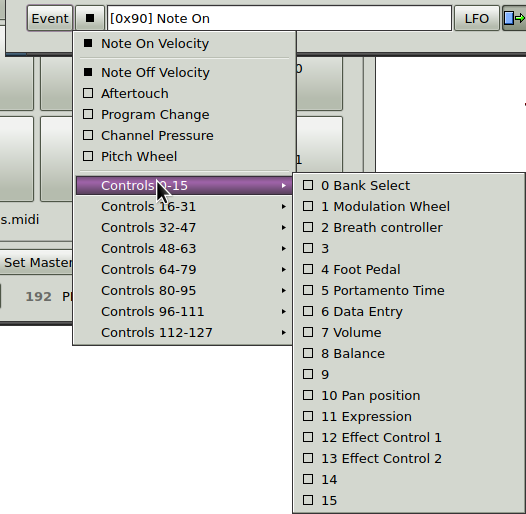
\includegraphics[scale=0.75]{pattern-editor/event-context-menu.png}
   \caption{Pattern Editor Event Button Context Menu}
   \label{fig:pattern_editor_bottom_event_context_menu}
\end{figure}

   Note the squares.  Some might be filled (black), most are empty.
   Filled squares indicate that the sequence has some events of that type.
   Otherwise, there are no such events in the sequence.
   Useful in deciding if it is worth selecting the event.

   The sub-menus of this context menu show 128 MIDI controller messages.
   They also use the squares to
   indicate if there are any events of the type shown in the menu.
   These sub-menus can be modified by editing the 'usr' file:
   
   \begin{verbatim}
      $HOME/.config/seq66/seq66.usr
   \end{verbatim}

   to make it match one's instrument.

   \itempar{Existing Event Menu}{pattern editor!existing events}
   The existing-event selector is a small button (with a black-square icon)
   that brings up a menu with only existing events shown.
   Unlike the event-selector described above, this menu
   shows only the actual events existing in the track, for quicker selection.

   \itempar{Event Selection}{pattern editor!event selection}
   Shows the selection event, with its event number shown in hexadecimal
   notation, and the name of the event shown.

   \itempar{LFO Panel}{pattern editor!LFO}
   An LFO (low-frequency oscillator) allows data events
   to be modulated by some rudimentary wave functions.
   By clicking on the \textbf{LFO} button or using the \texttt{Ctrl-L} key,
   the following window appears, with a set of 4 vertical sliders:

\begin{figure}[H]
   \centering 
  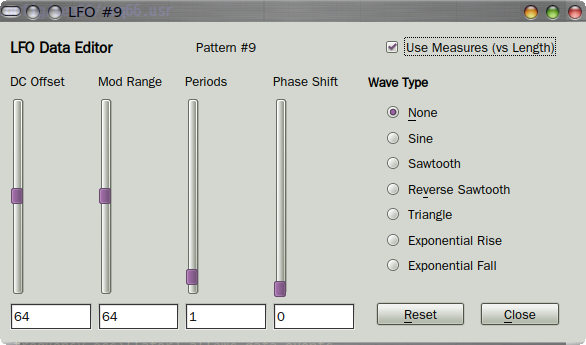
\includegraphics[scale=0.65]{pattern-editor/lfo.png}
   \caption{Pattern Editor LFO}
   \label{fig:pattern_editor_bottom_lfo}
\end{figure}

%  Note the controls in this window:

   \begin{enumber}
      \item \textbf{Use Measures (vs Length)}.
         The length of a waveform period can be determined by the length of the
         pattern (2 measures as shown next to the label "LFO Data Editor") or
         by the length of a measure. This check-box determines that.
         In the diagram, it is checked, so the 2 measures covers four periods
         of the sine wave.
         Especially useful in modifying long patterns.
      \item \textbf{DC Offset} (\textbf{D}).
         Provides a kind of DC offset for the data value. Starts at 64, and
         ranges from 0 to 127.
         In the diagram above, one can see that the 0-value line for the sine
         wave is at 64.
      \item \textbf{Mod Range} (\textbf{R}).
         Controls the depth of modulation. Starts at 64, and ranges from 1 to
         127.
         The data values range from \( y = DC - R \) to \( y = DC + R\).
         For the sine-wave shown above, the range is 0 to 128 (actually 127).
      \item \textbf{Periods}.
         Indicates the number of periods per pattern length.
         For long patterns, this parameter should be set high,
         to even show an effect.  It is also subject to an 'anti-aliasing'
         effect, especially for short patterns.
         Try it!
      \item \textbf{Phase Shift} (\textbf{P}).
         Provides the phase shift within a period of the LFO wave.
         A value of 1 is a phase shift of 360 degrees (one whole period).
         Thus, the data at \( P = 0 \) would look exactly the same at phase
         \( P = 1\).
      \item \textbf{Wave Type}.
         Selects the kind of wave to use for the LFO:
         \begin{enumber}
            \item \textbf{None}.
               This setting is useful if one wants to change only the DC
               offset.
            \item \textbf{Sine}.  Modulates via a sine wave.
            \item \textbf{Sawtooth}. Provides a ramp modulation.
            \item \textbf{Reverse Sawtooth}. Provides a ramp modulation in the
               opposite direction.
            \item \textbf{Triangle}. Modulates via a triangle wave; somewhat
               similar to a sine wave.
         \end{enumber}
         Note that one might have to change a parameter slightly to see the
         effect of the new waveform.
      \item \textbf{Reset Data}.
         This button restores the initial pattern event data.  Useful when one
         applies modulation that one ultimately does not like.
      \item \textbf{Close}.  Closes the LFO panel.
   \end{enumber}

   In addition to the \textbf{Reset Data} button, Ctrl-Z can be applied
   multiple times to undo changes one at a time.  Every motion of a control
   causes a complete change.

   \itempar{Live Loop Count}{pattern editor!live loop count}
   Normally, in Live mode, a pattern plays endlessly if left alone.
   If this counter is set to a value greater than 0, then the pattern will loop
   only that number of times in Live mode.  For example, if set to 1, then the
   pattern acts like a "one-shot" loop.  This can save having to use
   queuing quickly to handle an intro phrase.
   To loop \textsl{endlessly}, set this value to 0.

   \itempar{Armed/Mute Toggle}{pattern editor!data to midi buss}
   This button causes the pattern to be output to the
   selected MIDI output buss,
   which will normally be connected to a software or hardware
   synthesizer, to be heard.
   This item performs muting/unmuting (disarming/arming) in the same way a
   pressing the corresponding pattern button in the \textbf{Live} frame.

   \itempar{MIDI Thru Toggle}{pattern editor!midi data pass-through}
   This button routes incoming MIDI data through
   \textsl{Seq66}, which then writes it to the MIDI output buss.
   When a new pattern editor is opened,
   and the new-editor-editor settings
   (\sectionref{paragraph:user_file_added_options_pattern_editor})
   are false, one can click the
   \index{thru}
   \textbf{Thru} button first to redirect MIDI controller input
   to the synthesizer port, and have it be heard, without
   arming the pattern or turning on MIDI Record.

   Note, though, that if MIDI Record is toggled on and off, the
   Thru function is effectively disabled.  To restore it,
   toggle the Thru off, then on, again.

   Also note that Thru will remain enabled when the pattern editor is closed.

   \itempar{MIDI Record Toggle}{pattern editor!record midi data}
   This button routes incoming MIDI data into
   \textsl{Seq66}, which then saves the data to its buffer, and also
   displays the new information (notes) in the piano roll view.

   \itempar{MIDI Record Quantized}{pattern editor!quantized record}
   This button will causes MIDI data to be recorded, but be
   quantized on the fly before recording it.
   The quantization is to the current snap value.

   \itempar{Loop Record Type}{pattern editor!recording type}
   In \textsl{Seq24}, the pattern recording worked by merging new notes played
   as the pattern to be recorded was looped.  This method allows a loop to be
   built up bit-by-bit.  \textsl{Seq66} adds two more methods from
   Stazed's \textsl{Seq32} project.  The three methods are:

   \begin{enumber}
      \item \textbf{Merge}.
         \index{merge}
         \index{recording type!merge}
         This is the normal style of recording loops, where notes can
         accumulate as the loop repeats.
      \item \textbf{Replace.}
      \index{replace}
      \index{recording type!replace}
         When the loop starts over, and a note is pressed,
         then the existing notes in that loop are erased,
         and the new note is added.
         This provides a good way of correcting major mistakes, live.
         It will not work if adding notes while not recording.
         This mode can cause incomplete notes if one
         holds the note and releases it in the next iteration, leaving a
         partially-drawn note behind.  The workaround is to try again.
      \item \textbf{Expand}.
         \index{expand}
         \index{recording type!expand}
         Once the end of the loop is near, whether or
         not any notes are being input, another measure is added to the length
         of the loop.
         This continues indefinitely, whether or not any notes are
         being played/recorded.
      \item \textbf{Oneshot}.
         \index{oneshot}
         \index{recording type!oneshot}
         When this option is set, with the record button on, and no pattern
         playing, recording won't start until a note comes in, and when the
         first note comes in, the progress bar starts at the left (time 0).
         As each new set of notes at the same timestamp come in, the
         notes are recorded and the current time advances by one snap value.
         At the end of the pattern, recording stops automatically.
         See the figure
         below for a recording from a \textsl{Yamaha DD-11}.
         The length of each note is determined by the snap size for the spacing
         of drawn events.
   \end{enumber}

\begin{figure}[H]
   \centering 
   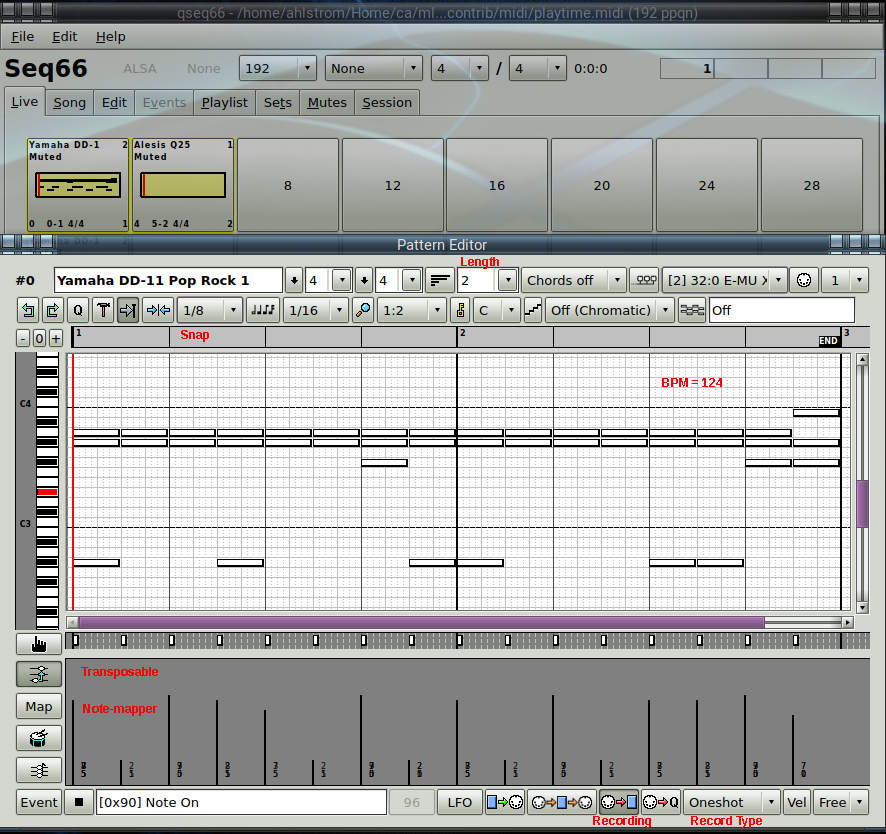
\includegraphics[scale=0.65]{pattern-editor/oneshot-recording.png}
   \caption{One-Shot Pattern Recording}
   \label{fig:pattern_editor_oneshot_recording}
\end{figure}

   In the figure above, we set up to record input from the port attached to a
   \textsl{Yamaha DD-11} drum machine.  After some trial and error,
   we set the \textbf{Length} to 2 measures (see the red text); the
   \textbf{Snap} to 1/8th; the \textbf{Recording Type} to "Oneshot"; and
   \textbf{Recording} on; also, the \textbf{BPM} was set to 124 in the main
   window, to match the "39" tempo in the DD-11, which maps to 124 bpm.
   Finally, we picked the \textsl{Pop Rock 1} style.  
   Once this setup was in place, clicking the DD-11 Start/Stop button started
   recording automatically at time 0, and it stopped automatically at the
   length/end of the pattern.

   Why is the snap used instead of the note-length?  Because we're using the
   \index{auto-step}
   \index{step-edit}
   auto-step (step-edit) feature... the snap determines where the next note
   begins, and the length determines the length of the note to create.
   However, the note-length is a property of the piano roll, not the pattern
   itself.  The pattern uses the snap-length during auto-step.

   Now, the DD-11 is an old instrument from the pre-General-MIDI days.
   So, in order to play back this pattern on something like
   \textsl{QSynth} or \textsl{Hydrogen}, we need to re-map the notes to GM drum
   notes.  In the 'rc' file, the proper note-mapper file is specified:

   \begin{verbatim}
      [note-mapper]
      "GM_DD-11.drums"
   \end{verbatim}

   We copy the recorded pattern and paste it into another slot for safety.
   We click the \textbf{Transposable} button for that pattern to enable the
   \textbf{Map} button.  Then we click the \textbf{Map} button, and the notes
   shift (not shown).  
   We click the \textbf{Transposable} button again to disable transposing,
   and save the file.
   Playing it into channel 10 of \textsl{QSynth} shows that it sounds a lot
   like the original DD-11 drums.

   \itempar{Vol}{pattern editor!vol}
   This button resets the volume (velocity)
   of note recording to the \textbf{Free} setting.
   See the next item.

   \itempar{Velocity}{pattern editor!velocity}
   This dropdown allows setting the volume of the recording to either the
   incoming velocity or to the specified velocity.
   The velocity values are shown at the right side of each menu entry.
   These values correspond to MIDI volume levels from 127 down to 16.
   If the \textbf{Free} item is selected, then the incoming note velocity is
   preserved.

\subsection{Pattern Editor / Common Actions}
\label{subsec:pattern_editor_common}

   This section is a catch-all for actions not described above.

\subsubsection{Pattern Editor / Common Actions / Scrolling}
\label{subsec:pattern_editor_scrolling}

   \textsl{We still need to work out whether or not to use the scroll wheel.
   in Seq66, as we need to keep multiple event panes in sync while scrolling.}

   Let us describe the actions that can be performed with a
   scroll wheel, or with the scrolling features of multi-touch touchpads.
   There are three major scrolling actions available when using mouse
   scrolling, with the mouse hovering in the piano-roll area:

   \begin{itemize}
      \item \textbf{Vertical Panning (Notes Panning)}
         \index{scroll!normal scroll}
         \index{scroll!vertical pan}
         \index{scroll!notes pan}
         \index{pan!seqroll notes}
         Using the vertical scroll action of a mouse or touchpad moves the
         view of the sequence/pattern notes up and down.
         One can also click in the piano roll, and then use the
         \texttt{Page-Up} \index{keys!page-up}
         and \texttt{Page-Down} \index{keys!page-down}
         keys to move the view up and down in pitch.
      \item \textbf{Horizontal Panning (Timeline Panning)}
         \index{scroll!shift scroll}
         \index{scroll!horizontal pan}
         \index{scroll!timeline pan}
         \index{pan!seqroll time}
         Holding the Shift key, and then using the vertical scroll action of a
         mouse or touchpad moves the view of the sequence/pattern time forward
         and backward.
         One can also click in the piano roll, and then use the
         \texttt{Shift Page-Up} \index{keys!shift page-up}
         and \texttt{Shift Page-Down} \index{keys!shift page-down}
         keys to move the view left and right in time.
      \item \textbf{Horizontal Zoom (Timeline Zoom)}
         \index{scroll!ctrl scroll}
         \index{scroll!horizontal zoom}
         \index{scroll!timeline zoom}
         \index{zoom!seqroll time}
         Holding the Ctrl key, and then using the vertical scroll action of a
         mouse or touchpad zooms the view of the sequence/pattern time to
         compress it or expand it.
         One can also click in the piano roll, and then use the
         \texttt{z} \index{keys!z},
         \texttt{Z} \index{keys!Z}, and
         \texttt{0} \index{keys!0} keys to change the timeline zoom.
      \item \textbf{Vertical Zoom (Notes Zoom)}
         \index{scroll!vertical zoom}
         \index{scroll!notes zoom}
         \index{zoom!seqroll notes}
         Additional buttons for vertical zoom have been added:
         \textbf{-},
         \textbf{0}, and
         \textbf{+}.
         One can also click in the piano roll, and then use the
         \texttt{v} \index{keys!v},
         \texttt{V} \index{keys!V}, and
         \texttt{0} \index{keys!0} keys to change the notes zoom.
         The zoom can make the note-rows large enough to use on a touch screen.
   \end{itemize}

   The actions of this scrolling are smooth and fast.
   If an event is selected in the piano-roll area or the (thin) event area,
   then the scrolling increases or decreases the value of the event.
   In the case of a note, this increases or decreases the velocity of the note.
   For all events, this increases or decreases the length of the vertical line
   that represents the value of the event.

\subsubsection{Pattern Editor / Common Actions / Close}
\label{subsec:pattern_editor_close}

   \index{window!close}
   There is no \textbf{Close} button in the pattern editor.  One can use
   window-manager actions, such as clicking on the \textbf{X}
   button of the window
   frame, or pressing the exit key defined in the window manager.

%-------------------------------------------------------------------------------
% vim: ts=3 sw=3 et ft=tex
%-------------------------------------------------------------------------------
